\section{Experimental results}
\label{sec:results}

This section presents experimental results which demonstrate the value
of Prairie in specifying rule sets of rule-based optimizers.  Our
experiments consist of specifying rule-based optimizers using Prairie
and generating optimizers using the P2V pre-processor and the
optimizer-generator paradigm of Figure~\ref{fig:ptovmodel}.

In \cite{Das93}, we presented an implementation of a centralized
relational query optimizer using Prairie.  Using the P2V translator, we
translated this to Volcano format and optimized several queries using
the resultant optimizer.  For comparison, we hand-coded the same
optimizer directly in Volcano.  The results presented there showed
that, using Prairie (compared to directly using Volcano) resulted in
approximately 50\% savings in lines of code with negligible (less than
5\%) increase in query optimization time.  However, the optimizer was
quite small in terms of the number of operators, algorithms and rules.

For a more realistic evaluation of Prairie, we needed answers to
the following questions:
\begin{enumerate}
\item Is Prairie adequate for large-scale rule sets?
\item How is programmer productivity enhanced by the high-level
      abstractions of Prairie?
\item Can Prairie rule sets be translated automatically into
      efficient implementations?
\end{enumerate}

We addressed the first question by using the Texas Instruments Open
OODB query optimizer rule set, which has the largest publicly
available rule set.  We describe this optimizer in the next section,
and then give our assessments to the last two questions in subsequent
sections.

\subsection{The Texas Instruments Open OODB query optimizer}
\label{sec:oodb}

The Texas Instruments Open Object-Oriented Database Management System
is an open, extensible, object-oriented database system which provides
users an architectural framework that is configurable in an incremental
manner.  The query optimizer in the Open OODB \cite{Blak93} is
generated using Volcano.  It is written as a set of trans\_rules and
impl\_rules that define the algebra of an object-oriented database
system.  Currently, there are 17 transformation rules and 9
implementation rules together with about $13,000$ lines of code for
support functions; this, of course, can be changed by an Open OODB user
for specific needs.

\subsection{Programmer productivity}
\label{sec:productivity}

Programmer productivity can be measured in different ways.  An
admittedly simplistic metric is the number of lines of code that must
be written.  But there are also less tangible measures, such as the
amount of conceptual effort needed to understand a particular
programming task.  Our experience with the Open OODB query optimizer
suggests that Prairie excels on the latter, while offering modest
reductions in the volume of code that needs to be written.

We converted by hand the Open OODB query optimizer's Volcano
specifications to Prairie.  This was a non-trivial task because of the
relatively large size of the rule set and the complexity of the support
functions.  This was where we found Prairie helped in conceptually
simplifying the rules and actions.  We then used our P2V pre-processor
to reconstitute these Prairie specifications as Volcano
specifications.  As described in Section~\ref{sec:ptov}, this process
involved a considerable level of complexity, partly because the Prairie
specification had 22 T-rules and 11 I-rules compared to 17 trans\_rules
and 9 impl\_rules in the Volcano specification; the reconstituted
Volcano specification had the same number of trans\_rules and
impl\_rules as the original hand-coded specification.

Converting the Open OODB optimizer rule set into Prairie format
actually simplified its specification as the complexities of the
Volcano model were removed.  The reduction in lines of code was modest
--- there was about a 10\% savings.\footnote{The original Volcano
specification had $13,400$ lines, the Prairie specification had
$12,100$ lines, and the P2V-generated Volcano specification had
$15,800$ lines.} However, as mentioned above, savings in lines of code
do not adequately reflect increases in programmer productivity.  We
found the encapsulated specifications of Prairie --- namely, the use of
a single descriptor and fewer explicit support functions --- made rule
programming \emph{much} easier.

\subsection{Performance results using the Open OODB optimizer}
\label{sec:oodbexp}

\newsavebox{\Eone}
\newsavebox{\Etwo}
\newsavebox{\Ethree}
\newsavebox{\Efour}

\begin{lrbox}{\Eone}
\begin{minipage}[b]{1.9cm}
\psset{unit=4mm}
\psset{nodesep=1pt}
\tiny
\begin{center}
\begin{pspicture}(0,0)(4,4)
\rput(0,0){\rnode{cl1}{$\textit{C}_1$}}
\rput(0,1){\rnode{getcl1}{RET}}
\ncline{-}{cl1}{getcl1}
\rput(2,0){\rnode{cl2}{$\textit{C}_2$}}
\rput(2,1){\rnode{getcl2}{RET}}
\ncline{-}{cl2}{getcl2}
\rput(1,2){\rnode{joingetcl1getcl2}{JOIN}}
\ncline{-}{joingetcl1getcl2}{getcl1}
\ncline{-}{joingetcl1getcl2}{getcl2}
\rput{45}(2,3){\rnode{dots}{$\ldots$}}
\ncline{-}{joingetcl1getcl2}{dots}
\rput(4,3){\rnode{getcln}{RET}}
\rput(4,2){\rnode{cln}{$\textit{C}_n$}}
\ncline{-}{cln}{getcln}
\rput(3,4){\rnode{root}{JOIN}}
\ncline{-}{root}{dots}
\ncline{-}{root}{getcln}
\end{pspicture}
\end{center}
\end{minipage}
\end{lrbox}

\begin{lrbox}{\Etwo}
\begin{minipage}[b]{1.9cm}
\psset{unit=4mm}
\psset{nodesep=1pt}
\tiny
\begin{center}
\begin{pspicture}(0,0)(4,5)
\rput(0,0){\rnode{cl1}{$\textit{C}_1$}}
\rput(0,1){\rnode{getcl1}{RET}}
\ncline{-}{cl1}{getcl1}
\rput(2,0){\rnode{cl2}{$\textit{C}_2$}}
\rput(2,1){\rnode{getcl2}{RET}}
\ncline{-}{cl2}{getcl2}
\rput(0,2){\rnode{matgetcl1}{MAT}}
\ncline{-}{getcl1}{matgetcl1}
\rput(2,2){\rnode{matgetcl2}{MAT}}
\ncline{-}{getcl2}{matgetcl2}
\rput(1,3){\rnode{joinmatgetcl1matgetcl2}{JOIN}}
\ncline{-}{joinmatgetcl1matgetcl2}{matgetcl1}
\ncline{-}{joinmatgetcl1matgetcl2}{matgetcl2}
\rput{45}(2,4){\rnode{dots}{$\ldots$}}
\ncline{-}{joinmatgetcl1matgetcl2}{dots}
\rput(4,3){\rnode{getcln}{RET}}
\rput(4,2){\rnode{cln}{$\textit{C}_n$}}
\ncline{-}{cln}{getcln}
\rput(4,4){\rnode{matgetcln}{MAT}}
\ncline{-}{matgetcln}{getcln}
\rput(3,5){\rnode{root}{JOIN}}
\ncline{-}{root}{dots}
\ncline{-}{root}{matgetcln}
\end{pspicture}
\end{center}
\end{minipage}
\end{lrbox}

\begin{lrbox}{\Ethree}
\begin{minipage}[b]{1.9cm}
\psset{unit=4mm}
\psset{nodesep=1pt}
\tiny
\begin{center}
\begin{pspicture}(0,0)(4,5)
\rput(0,0){\rnode{cl1}{$\textit{C}_1$}}
\rput(0,1){\rnode{getcl1}{RET}}
\ncline{-}{cl1}{getcl1}
\rput(2,0){\rnode{cl2}{$\textit{C}_2$}}
\rput(2,1){\rnode{getcl2}{RET}}
\ncline{-}{cl2}{getcl2}
\rput(1,2){\rnode{joingetcl1getcl2}{JOIN}}
\ncline{-}{joingetcl1getcl2}{getcl1}
\ncline{-}{joingetcl1getcl2}{getcl2}
\rput{45}(2,3){\rnode{dots}{$\ldots$}}
\ncline{-}{joingetcl1getcl2}{dots}
\rput(4,3){\rnode{getcln}{RET}}
\rput(4,2){\rnode{cln}{$\textit{C}_n$}}
\ncline{-}{cln}{getcln}
\rput(3,4){\rnode{root}{JOIN}}
\ncline{-}{root}{dots}
\ncline{-}{root}{getcln}
\rput(3,5){\rnode{select}{SELECT}}
\ncline{-}{select}{root}
\end{pspicture}
\end{center}
\end{minipage}
\end{lrbox}

\begin{lrbox}{\Efour}
\begin{minipage}[b]{1.9cm}
\psset{unit=4mm}
\psset{nodesep=1pt}
\tiny
\begin{center}
\begin{pspicture}(0,0)(4,6)
\rput(0,0){\rnode{cl1}{$\textit{C}_1$}}
\rput(0,1){\rnode{getcl1}{RET}}
\ncline{-}{cl1}{getcl1}
\rput(2,0){\rnode{cl2}{$\textit{C}_2$}}
\rput(2,1){\rnode{getcl2}{RET}}
\ncline{-}{cl2}{getcl2}
\rput(0,2){\rnode{matgetcl1}{MAT}}
\ncline{-}{getcl1}{matgetcl1}
\rput(2,2){\rnode{matgetcl2}{MAT}}
\ncline{-}{getcl2}{matgetcl2}
\rput(1,3){\rnode{joinmatgetcl1matgetcl2}{JOIN}}
\ncline{-}{joinmatgetcl1matgetcl2}{matgetcl1}
\ncline{-}{joinmatgetcl1matgetcl2}{matgetcl2}
\rput{45}(2,4){\rnode{dots}{$\ldots$}}
\ncline{-}{joinmatgetcl1matgetcl2}{dots}
\rput(4,3){\rnode{getcln}{RET}}
\rput(4,2){\rnode{cln}{$\textit{C}_n$}}
\ncline{-}{cln}{getcln}
\rput(4,4){\rnode{matgetcln}{MAT}}
\ncline{-}{matgetcln}{getcln}
\rput(3,5){\rnode{root}{JOIN}}
\ncline{-}{root}{dots}
\ncline{-}{root}{matgetcln}
\rput(3,6){\rnode{select}{SELECT}}
\ncline{-}{select}{root}
\end{pspicture}
\end{center}
\end{minipage}
\end{lrbox}

\begin{centeredfigure*}
\begin{minipage}[b]{9.1cm}
\myshadowbox{
\begin{minipage}[b]{8.6cm}
\subfigure[E1] { \usebox{\Eone} \label{fig:Eone} }
\vrule
\subfigure[E2] { \usebox{\Etwo} \label{fig:Etwo} }
\vrule
\subfigure[E3] { \usebox{\Ethree} \label{fig:Ethree} }
\vrule
\subfigure[E4] { \usebox{\Efour} \label{fig:Efour} }
\normalsize
\end{minipage}
}
\caption{Expressions used in generating queries for experiments}
\label{fig:exps}
\end{minipage}
\hfill
\begin{minipage}[b]{7.0cm}
% Save current figure counter
\newcounter{savectr}
\setcounter{savectr}{\value{figure}}
% Temporarily change the figure to a table.
\renewcommand{\figurename}{\tablename}
\setcounter{figure}{\value{table}}
\scriptsize
\renewcommand{\multirowsetup}{\centering}
\newlength{\Lone}
\settowidth{\Lone}{E4}
\newlength{\Ltwo}
\settowidth{\Ltwo}{\textbf{Query}}
\newlength{\Lthree}
\settowidth{\Lthree}{\textbf{Indices?}}
\newlength{\Lfour}
\settowidth{\Lfour}{\textbf{Expression}}
\newlength{\Lnum}
\settowidth{\Lnum}{99}
\begin{tabular}{|c|c|c|c|c|} \thickhline
\multirow{2}{\Ltwo}{\textbf{Query}}
  & \multirow{2}{\Lthree}{\textbf{Indices?}}
  & \multirow{2}{\Lfour}{\textbf{Expression}} 
  & \multicolumn{2}{c|}{\textbf{Rules matched}} \\ \cline{4-5}
& & & trans\_rules & impl\_rules \\ \thickhline
Q1 & No & \multirow{2}{\Lone}{E1} & \multirow{2}{\Lnum}{3}
  & \multirow{2}{\Lnum}{3} \\ \cline{1-2}
Q2 & Yes & & & \\ \hline
Q3 & No & \multirow{2}{\Lone}{E2} & \multirow{2}{\Lnum}{8}
  & \multirow{2}{\Lnum}{4} \\ \cline{1-2}
Q4 & Yes & & & \\ \hline
Q5 & No & \multirow{2}{\Lone}{E3} & \multirow{2}{\Lnum}{9}
  & \multirow{2}{\Lnum}{5} \\ \cline{1-2}
Q6 & Yes & & & \\ \hline
Q7 & No & \multirow{2}{\Lone}{E4} & \multirow{2}{\Lnum}{16}
  & \multirow{2}{\Lnum}{7} \\ \cline{1-2}
Q8 & Yes & & & \\ \thickhline
\end{tabular}
\caption{Queries used in experiments}
\label{tab:queries}
% Change figure back as usual.
\renewcommand{\figurename}{Figure}
\setcounter{figure}{\value{savectr}}
\end{minipage}
\end{centeredfigure*}

The acid test of Prairie was whether Prairie specifications could be
translated into efficient optimizer implementations.  Our experiments
using the Open OODB consisted of optimizing 8 different queries using
the two query optimizers generated, respectively, using Prairie and
using Volcano directly (in the remainder of this section, we will use
``Prairie'' and ``Volcano'' to denote these two approaches).  There
were 4 distinct expressions that were used to generate the queries used
in the experiments; these are shown in Figure~\ref{fig:exps}.  Each
expression represents an $N$-way join query for varying $N$.

The first expression E1 is a simple retrieval and join of base
classes.  The second, E2, is also a join of base classes; however,
after each class retrieval, an attribute has to be materialized (\ie
brought into view) before the join.  The third and fourth expressions
(E3 and E4) are the same as the first and second (E1 and E2)
respectively, except that there is a selection of attributes (the
select operator is the root of the expressions).\footnote{ The most
complex expression E4 consists of all operators in the algebra, except
PROJECT and UNNEST.  PROJECT was not considered because it appeared in
only one impl\_rule and no trans\_rules, and thus, would not affect the
size of the search space of abstract expressions.  UNNEST was not
considered because it appeared in exactly one trans\_rule and one
impl\_rule; including it in our queries would have increased the number
of parameters that could affect our run-times.  We preferred to
concentrate on simple JOIN expressions.}

The algebra that was used in the Prairie and Volcano optimizers for our
experiments consisted of 5 relational operators SELECT, PROJECT, JOIN,
RET and UNNEST (for set-valued attributes) and an object-oriented
operator called MAT (for MATerialize; it is fundamentally a
pointer-chasing operator for attributes of a class).  There were 8
algorithms.

There are many parameters that can be varied when benchmarking a query
optimizer.  Since our objective was to verify that the Prairie approach
did not sacrifice efficiency, our criteria for the queries was that
they test a majority of the rules, with varying properties of the base
classes.  To this end, we tested our optimizer (and the Volcano
optimizer) with 8 different queries (shown in Table~\ref{tab:queries}).
The eight queries Q1 through Q8 are derived from the 4 expressions in
Figure~\ref{fig:exps}.  Each expression E1 through E4 is used to obtain
two queries for a fixed number $N$ of JOINs in the expression.  The
only difference between the two queries obtained from an expression is
that the first one does not contain any indices on any classes, whereas
the second one contains a single index on each base class occurring in
the expression.  In expressions where a SELECT is present (E3 and E4),
the selection predicate is a conjunction of equality predicates
$\textit{bc}_i == \textit{const}_i$, where $\textit{bc}_i$ is an
attribute of class $\textit{C}_i$, and $\textit{const}_i$ is a constant
(we arbitrarily set this to $i$, because its value doesn't affect the
correctness or performance of the optimizer).  In addition, for queries
with a SELECT and whose base classes have indices (Q6 and Q8 in
Table~\ref{tab:queries}), the (single) index of each base class was
chosen to be the attribute referenced in the selection predicate.  For
example, class $\textit{C}_i$ was chosen to have an index on attribute
$\textit{bc}_i$.  The join predicates for each JOIN were chosen at
random, and were always equality predicates.  The choice of JOIN
predicates was such that the queries corresponded to linear query
graphs.  In the future, we will experiment with non-linear (\eg star)
query graphs.

Table~\ref{tab:queries} also shows the number of trans\_rules and
impl\_rules that are matched by each expression.  These are the rules
whose left hand sides match a sub-expression.  However, not all the
rules were necessarily applicable.  For instance, an impl\_rule with an
index scan would not apply to Q3, although it might apply to Q4.

Queries Q1 through Q8 were optimized for increasing number $N$ of
JOINs.  For a fixed number of JOINs in a query, we varied the
cardinalities of the base classes 5 times, each time generating a query
with different class properties, and averaged the run-times over the 5
query instances to generate the per-query optimization time.  Thus,
each point in our graphs represents the average of 5 queries.  The
run-times were measured\footnote{Since the run-times were too small to
be measured accurately with \texttt{time}, each query instance was
optimized 3000 times (in a loop) and the total time was divided by 3000
to get the per-query optimization time.} using the GNU \texttt{time}
command.  All experiments were performed on a lightly loaded DECstation
5000/200 running Ultrix 4.2.

The optimization times for each query for both approaches (Prairie and
Volcano) are shown in Figures~\ref{fig:q1} through \ref{fig:q8}.  The
number of joins in each set of graphs was varied to a maximum of 8, or
until virtual memory was exhausted.

The first set of graphs (Figures~\ref{fig:q1} and \ref{fig:q2})
shows the performance of a simple relational-type query.  The
optimization times are almost identical between Prairie and Volcano,
and the notable point is that the presence of an index does not change
the optimizer's behavior, \ie the two graphs are identical.  This
arises because the optimizer algebra had only two join algorithms
(pointer join and hash join), neither of which makes use of any
indices.

The second set of graphs (Figures~\ref{fig:q3} and \ref{fig:q4}) shows
the results of optimizing Q3 and Q4.  Here, as in Figures~\ref{fig:q1}
and \ref{fig:q2}, the presence (or absence) of indices makes no
difference.  Both the Prairie and Volcano approaches have comparable
run-times.  The sharp jump in the graphs from 7-way to 8-way joins is
due to the fact that since all optimization is done in main memory,
dynamic memory allocation (caused by \texttt{malloc} calls) results in
a lot of thrashing at this point.  We speculate that in systems with
more virtual memory, the graphs will be smoother.

The third and fourth sets of graphs in Figures~\ref{fig:q5} through
\ref{fig:q8} are optimizations of queries with a selection predicate.
In these cases, the presence of an index makes a difference if the
index is referenced in the selection predicate (as we designed).  Also,
in these two figures, the performance of both Prairie and Volcano was
almost identical, except that Prairie does slightly worse due to the
larger number of \texttt{malloc} calls that the P2V translator
introduces.  Also, note that we could only go up to 3-way joins before
virtual memory was exhausted.  As the available memory decreases, there
is increased thrashing (as shown by the sharp changes in slope in the
plots) resulting in a much slower optimization process.

\begin{centeredfigure}
\myshadowbox
{
\setlength{\tabcolsep}{0pt}
\begin{tabular}{ll}
\subfigure[Query 1] { \begin{centeredinhalfminipage}
                      \vspace{3mm}
                      \epsfig{file=runtime_Q1.ps,width=3.0cm}
                      \end{centeredinhalfminipage}
                      \label{fig:q1} }
&
\subfigure[Query 2] { \begin{centeredinhalfminipage}
                      \vspace{3mm}
                      \epsfig{file=runtime_Q2.ps,width=3.0cm}
                      \end{centeredinhalfminipage}
                      \label{fig:q2} }
\\ \hline
\subfigure[Query 3] { \begin{centeredinhalfminipage}
                      \vspace{4mm}
                      \epsfig{file=runtime_Q3.ps,width=3.0cm}
                      \end{centeredinhalfminipage}
                      \label{fig:q3} }
&
\subfigure[Query 4] { \begin{centeredinhalfminipage}
                      \vspace{4mm}
                      \epsfig{file=runtime_Q4.ps,width=3.0cm}
                      \end{centeredinhalfminipage}
                      \label{fig:q4} }
\\ \hline
\subfigure[Query 5] { \begin{centeredinhalfminipage}
                      \vspace{4mm}
                      \epsfig{file=runtime_Q5.ps,width=3.0cm}
                      \end{centeredinhalfminipage}
                      \label{fig:q5} }
&
\subfigure[Query 6] { \begin{centeredinhalfminipage}
                      \vspace{4mm}
                      \epsfig{file=runtime_Q6.ps,width=3.0cm}
                      \end{centeredinhalfminipage}
                      \label{fig:q6} }
\\ \hline
\subfigure[Query 7] { \begin{centeredinhalfminipage}
                      \vspace{4mm}
                      \epsfig{file=runtime_Q7.ps,width=3.0cm}
                      \end{centeredinhalfminipage}
                      \label{fig:q7} }
&
\subfigure[Query 8] { \begin{centeredinhalfminipage}
                      \vspace{4mm}
                      \epsfig{file=runtime_Q8.ps,width=3.0cm}
                      \end{centeredinhalfminipage}
                      \label{fig:q8} }
\end{tabular}
}
\caption{Query optimization times for Q1 through Q8}
\label{fig:e4}
\end{centeredfigure}

In all four sets of plots, we can see that Prairie performs with almost
(less than $5\%$ variation) the same efficiency as Volcano.  In extreme
cases, when memory is scarce, Prairie runs more slowly (about $15\%$)
(\eg Figure~\ref{fig:q6}), but we believe that this situation already
represents a serious bottleneck for both Volcano and Prairie.

The results presented in this section show that Prairie optimizers
need not sacrifice efficiency for clarity, even for large rule sets.
More research and validation is necessary to verify that Prairie is
an efficient tool for optimizer specification.
